% Options for packages loaded elsewhere
\PassOptionsToPackage{unicode}{hyperref}
\PassOptionsToPackage{hyphens}{url}
\documentclass[
]{article}
\usepackage{xcolor}
\usepackage{amsmath,amssymb}
\setcounter{secnumdepth}{-\maxdimen} % remove section numbering
\usepackage{iftex}
\ifPDFTeX
  \usepackage[T1]{fontenc}
  \usepackage[utf8]{inputenc}
  \usepackage{textcomp} % provide euro and other symbols
\else % if luatex or xetex
  \usepackage{unicode-math} % this also loads fontspec
  \defaultfontfeatures{Scale=MatchLowercase}
  \defaultfontfeatures[\rmfamily]{Ligatures=TeX,Scale=1}
\fi
\usepackage{lmodern}
\ifPDFTeX\else
  % xetex/luatex font selection
\fi
% Use upquote if available, for straight quotes in verbatim environments
\IfFileExists{upquote.sty}{\usepackage{upquote}}{}
\IfFileExists{microtype.sty}{% use microtype if available
  \usepackage[]{microtype}
  \UseMicrotypeSet[protrusion]{basicmath} % disable protrusion for tt fonts
}{}
\makeatletter
\@ifundefined{KOMAClassName}{% if non-KOMA class
  \IfFileExists{parskip.sty}{%
    \usepackage{parskip}
  }{% else
    \setlength{\parindent}{0pt}
    \setlength{\parskip}{6pt plus 2pt minus 1pt}}
}{% if KOMA class
  \KOMAoptions{parskip=half}}
\makeatother
\usepackage{longtable,booktabs,array}
\newcounter{none} % for unnumbered tables
\usepackage{calc} % for calculating minipage widths
% Correct order of tables after \paragraph or \subparagraph
\usepackage{etoolbox}
\makeatletter
\patchcmd\longtable{\par}{\if@noskipsec\mbox{}\fi\par}{}{}
\makeatother
% Allow footnotes in longtable head/foot
\IfFileExists{footnotehyper.sty}{\usepackage{footnotehyper}}{\usepackage{footnote}}
\makesavenoteenv{longtable}
\usepackage{graphicx}
\makeatletter
\newsavebox\pandoc@box
\newcommand*\pandocbounded[1]{% scales image to fit in text height/width
  \sbox\pandoc@box{#1}%
  \Gscale@div\@tempa{\textheight}{\dimexpr\ht\pandoc@box+\dp\pandoc@box\relax}%
  \Gscale@div\@tempb{\linewidth}{\wd\pandoc@box}%
  \ifdim\@tempb\p@<\@tempa\p@\let\@tempa\@tempb\fi% select the smaller of both
  \ifdim\@tempa\p@<\p@\scalebox{\@tempa}{\usebox\pandoc@box}%
  \else\usebox{\pandoc@box}%
  \fi%
}
% Set default figure placement to htbp
\def\fps@figure{htbp}
\makeatother
\setlength{\emergencystretch}{3em} % prevent overfull lines
\providecommand{\tightlist}{%
  \setlength{\itemsep}{0pt}\setlength{\parskip}{0pt}}
\usepackage{bookmark}
\IfFileExists{xurl.sty}{\usepackage{xurl}}{} % add URL line breaks if available
\urlstyle{same}
\hypersetup{
  pdftitle={A Smart Queue Management System for Modern Healthcare},
  hidelinks,
  pdfcreator={LaTeX via pandoc}}

\title{A Smart Queue Management System for Modern Healthcare}
\author{}
\date{}

\begin{document}
\maketitle
CSE-033 - Prince Segokgo

 CSE24-122 - Ronaldinho

CSE24-092 -Wabatsha

 CSE24-037 - MOATHODI

 
PROJECT REPORT

Botswana Accountancy College

\section{Table of Contents}\label{table-of-contents}

1. Introduction

1.1 Problem Statement

1.2 Project Overview

1.3 Requirements

1.4 Documentation Structure

2. Background Literature

2.1 Introduction to Queue Management

2.2 Waiting Times in Healthcare

2.3 Digital Queue Management Systems

2.4 Mobile Technology and Digital Services in Botswana

2.5 Digital Transformation in Healthcare

2.6 Theoretical Framework: Technology Acceptance Model

2.7 Research Gap

2.8 Summary

3. Methodology and Analysis \& Design

3.1 Methodology

3.2 System Diagrams

3.3 Entity Relationship Diagram (ERD)

3.4 Class Diagrams

3.5 Dashboard Design

4. Implementation

5. Testing and Discussions

6. Conclusion

References

Appendices

Appendix A: Requirement Catalogue

Appendix B: Additional Material

\section{List of Figures}\label{list-of-figures}

Figure 1: QueLess System Context Diagram

Figure 2: QueLess Core Use Case Diagram

Figure 3: QueLess Entity Relationship Diagram

Figure 4: QueLess UML Class Diagram

Figure 5: QueLess Queue Joining and Notification Flow

Figure 6: Business Dashboard Wireframe

\section{Code Listing}\label{code-listing}

Listing 1: QueueManager responsibilities and queue-processing logic

Listing 2: NotificationService responsibilities

Listing 3: JoinQueueServlet request-handling logic (RQ01)

Listing 1: QueueManager.joinQueue() reserves the next queue position for
a user; callNextTicket() advances the queue and triggers RQ02
notification thresholds.

// QueueManager.java\\
public Ticket joinQueue(long queueId, String userName) \{\\
int nextPosition = tickets.values().stream()\\
.filter(t -\textgreater{} t.getQueueId() == queueId)\\
.mapToInt(Ticket::getPosition)\\
.max().orElse(0) + 1;\\
\strut \\
Ticket ticket = new Ticket(\\
ticketIdSeq.getAndIncrement(), queueId, userName, nextPosition);\\
tickets.put(ticket.getTicketId(), ticket);\\
return ticket;\\
\}\\
\strut \\
public void callNextTicket(long queueId) \{\\
Queue queue = queues.get(queueId);\\
if (queue == null) return;\\
getQueueStatus(queueId).stream().findFirst().ifPresent(front
-\textgreater{} \{\\
front.setStatus(Ticket.Status.SERVED);\\
queue.advanceServingPosition();\\
\});\\
evaluateNotificationThresholds(queueId,
queue.getCurrentServingPosition());\\
\}

Listing 2: NotificationService.sendPush() and notifyTurn() implement the
RQ02 notification thresholds (10 away, 2 away, and exact turn).

// NotificationService.java\\
public static final int NOTIFY\_FAR\_THRESHOLD = 10;\\
public static final int NOTIFY\_NEAR\_THRESHOLD = 2;\\
\strut \\
public void sendPush(Ticket ticket, int positionsAway) \{\\
ticket.setStatus(Ticket.Status.NOTIFIED);\\
ticket.setLastNotificationMessage(\\
"Your turn is approaching: " + positionsAway + " people ahead of
you.");\\
\}\\
\strut \\
public void notifyTurn(Ticket ticket) \{\\
ticket.setLastNotificationMessage(\\
"It is now your turn. Please proceed to the counter.");\\
\}

Listing 3: JoinQueueServlet.doPost() handles the RQ01 join-queue form
submission and redirects the user to their live status page.

// JoinQueueServlet.java\\
@WebServlet("/joinqueue")\\
public class JoinQueueServlet extends HttpServlet \{\\
\strut \\
protected void doPost(HttpServletRequest req, HttpServletResponse
resp)\\
throws ServletException, IOException \{\\
long queueId = Long.parseLong(req.getParameter("queueId"));\\
String userName = req.getParameter("userName");\\
if (userName == null \textbar\textbar{} userName.isBlank()) userName =
"Guest";\\
\strut \\
Ticket ticket = queueManager.joinQueue(queueId, userName);\\
resp.sendRedirect(req.getContextPath()\\
+ "/status?ticketId=" + ticket.getTicketId());\\
\}\\
\}

These excerpts are taken directly from the implemented QueLess web
application (queless-webapp Maven project, built with IntelliJ IDEA and
deployed to Apache Tomcat 11). The full source is included alongside
this report.

\section{1. Introduction}\label{introduction}

This section introduces the QueLess project. It presents the problem
being addressed, a brief overview of the proposed system, the high-level
requirements that guide the project, and the structure of the report.

\subsection{1.1 Problem Statement}\label{problem-statement}

Long queues at banks, clinics, government offices and retail shops
represent a daily source of frustration and lost productivity for people
living in Botswana. A primary research survey conducted with 50
participants found that 88 percent of respondents regularly experience
long queues in their daily lives, and this problem is echoed in
Botswana\textquotesingle s public healthcare system specifically, where
reports have documented overcrowding and extended waiting times at major
referral hospitals such as Princess Marina Hospital. At present, no
dedicated, locally built digital queue management solution exists for
the Botswana consumer market. Existing international queue management
systems are not adapted to local languages, currency or regulatory
requirements, leaving a clear gap between the scale of the problem and
the availability of a suitable local solution.

\subsection{1.2 Project Overview}\label{project-overview}

QueLess is a queue management system that allows users to join a service
queue digitally, reserving a position remotely and receiving real-time,
turn-based notifications as their position in the queue approaches. For
this stage of the project, QueLess is delivered as a Java web
application, accessed through a browser, so that both the user-facing
queue-joining screens and the business-facing dashboard can be
demonstrated and iterated on quickly; a native mobile application is
planned as a later-phase deliverable, as noted in Section 6.
Organisations use a companion QueLess business dashboard to manage and
monitor their queues. Together, these components are intended to remove
the need for individuals to stand in a physical line while giving
service providers greater visibility and control over how their queues
are managed. The initial focus of the project is the healthcare sector
in Botswana, with expansion into other service sectors planned for later
phases.

\subsection{1.3 Requirements}\label{requirements}

The requirements are divided into major requirements, which are
essential to the core function of QueLess, and minor requirements, which
extend or enhance that core function. The full catalogue is provided in
Appendix A.

\subsubsection{Major Requirements}\label{major-requirements}

The system shall allow a user to join a service queue remotely through a
web-based application, with a native mobile application planned for a
later phase.

The system shall notify a user in real time as their turn in the queue
approaches.

The system shall provide a business-facing dashboard through which an
organisation can create, manage and monitor its queues.

The system shall store user and queue data securely, in compliance with
the Botswana Data Protection Act (2018).

The system shall present its interface in both English and Setswana.

\subsubsection{Minor Requirements}\label{minor-requirements}

The system should provide an SMS-based notification option for users
without reliable smartphone data access.

The system should provide basic analytics for business subscribers, such
as queue-length trends and peak usage periods.

The system should support custom branding for enterprise-tier business
subscribers.

The system should allow API integration with an
organisation\textquotesingle s existing booking systems, for enterprise
clients.

\subsection{1.4 Documentation Structure}\label{documentation-structure}

Section 2 presents background literature relevant to queue management,
healthcare waiting times, digital queue systems, mobile technology in
Botswana, digital transformation in healthcare and the Technology
Acceptance Model. Section 3 presents the methodology and analysis and
design artefacts, including the system diagrams, ERD, UML class diagram
and dashboard wireframe. Section 4 describes the proposed implementation
architecture and technology stack. Section 5 defines the testing
strategy and discussion framework. Section 6 concludes the report and
identifies future work. References and appendices follow.

\section{2. Background Literature}\label{background-literature}

\subsection{2.1 Introduction to Queue
Management}\label{introduction-to-queue-management}

Queues form whenever the demand for a service temporarily exceeds the
capacity available to deliver it. This basic imbalance between arrivals
and service capacity is the foundation of queuing theory, which studies
how waiting occurs and how it can be managed. Beyond the mathematics of
arrival rates and service times, research has also turned to the human
experience of waiting. Maister (1985) argued that the perceived length
of a wait is often more important to a customer than its actual
duration, and identified principles such as the idea that unoccupied
time feels longer than occupied time, and that uncertain waits feel
longer than known, finite waits.

These psychological principles matter because long queues are widely
associated with negative outcomes for both customers and service
providers. Customers subjected to long or uncertain waits tend to report
frustration, anxiety and lower satisfaction with the service encounter,
while organisations experience congestion, reduced staff productivity
and a higher risk of losing customers who abandon the queue altogether
(Gokulakrishnan, 2023). This combination of a mathematical problem and a
psychological one is what makes queue management a subject of continuing
academic and practical interest, and it forms the starting point for
understanding why a digital solution such as QueLess is relevant.

\subsection{2.2 Waiting Times in
Healthcare}\label{waiting-times-in-healthcare}

Waiting times are a particularly well documented problem within
healthcare service delivery. McIntyre and Chow (2020) conducted a
narrative review of waiting times across primary care, emergency
departments, specialist referrals and elective procedures, and concluded
that waiting time is increasingly used as an indicator of how strained a
health system is, with longer waits generally associated with worse
patient outcomes and lower confidence in the health system. Similarly, a
large-scale survey of patients at primary health centres in Saudi Arabia
found a clear association between longer waiting times and lower patient
satisfaction, with patients who waited more than an hour significantly
more likely to report dissatisfaction than those seen within thirty
minutes (Alrasheedi et al., 2019).

Long waiting times in clinics and hospitals also contribute to
overcrowding, since patients who have already arrived continue to occupy
limited waiting-room space while new patients keep arriving. Garedew et
al. (2024) note that the healthcare sector is particularly prone to this
problem because it serves large and unpredictable patient volumes, which
leads to prolonged waiting times, overcrowding and, in some cases,
safety risks. Their study applied lean thinking and machine learning
techniques to a hospital setting specifically to reduce waiting time and
improve service quality, illustrating that healthcare providers
increasingly view waiting time as a measurable quality-improvement goal
rather than an unavoidable side effect of care delivery.

This problem is directly evident within Botswana\textquotesingle s own
public health system. A report by the Office of the Ombudsman, titled
Under Strain: Inside Botswana\textquotesingle s Public Health Care
Crisis, documented overcrowding, staff shortages and service breakdowns
at Princess Marina Hospital, the country\textquotesingle s main referral
hospital, and noted that most citizens live within five kilometres of a
health facility yet proximity alone does not guarantee timely treatment,
with patients often moving between clinics in search of shorter waits
(Office of the Ombudsman, cited in Daily News, 2026a). In response, the
Botswana government began converting the Sir Ketumile Masire Teaching
Hospital from a private to a fully public facility in 2026 specifically
to relieve congestion at Princess Marina, including expanding
orthopaedic bed capacity from 66 to 106 beds, at a time when about 800
patients were awaiting gynaecological surgery alone (Daily News, 2026b).
This local evidence confirms that the problem addressed by QueLess is
not only theoretical but is an active and recognised crisis within the
Botswana healthcare system.

\subsection{2.3 Digital Queue Management
Systems}\label{digital-queue-management-systems}

In response to the problems associated with physical queuing, service
organisations across many sectors have adopted digital or virtual queue
management systems. Rather than requiring customers to occupy a physical
line, these systems allow a customer to reserve a place in a queue
remotely, commonly through a mobile application, and to receive
real-time updates on their position and estimated waiting time. A study
of virtual queue management adoption among bank customers in Chennai
found that most users had begun to adopt the system because it was user
friendly, saved time, made services more accessible and increased
overall service efficiency compared with standing in a physical line
(Gokulakrishnan, 2023).

The core benefit of virtual queuing is that it separates a
customer\textquotesingle s place in the queue from their physical
presence in the waiting area. Customers can attend to other tasks while
waiting and are notified, typically by a mobile alert, when their turn
is approaching, which reduces the perceived burden of waiting described
by Maister (1985). For service providers, virtual queue management
systems also generate operational data that can be used to monitor
demand patterns, allocate staff more effectively and identify peak
periods, benefits that have been documented in educational, banking and
retail settings alike. These findings support the design logic behind
QueLess, which applies the same virtual-queuing principle to the
Botswana service sector, with an initial focus on healthcare.

\subsection{2.4 Mobile Technology and Digital Services in
Botswana}\label{mobile-technology-and-digital-services-in-botswana}

The feasibility of a mobile-based queue-management solution depends
heavily on the level of mobile technology adoption in the target market.
Botswana had an estimated population of about 2.6 million people in
2026, with 75.6 percent of that population living in urban areas and a
median age of only 23.7 years, characteristics generally associated with
faster technology adoption (Worldometer, 2026). DataReportal (2026)
recorded that 4.22 million cellular mobile connections were active in
Botswana by late 2025, equivalent to 164 percent of the total
population, a figure that exceeds the population itself due to
widespread multiple-SIM ownership. The same report found that 2.09
million individuals were using the internet by the end of 2025,
representing an internet penetration rate of 81.4 percent, while 1.40
million people held social-media user identities, equivalent to 54.4
percent of the population.

This growth is supported by improving infrastructure. Fixed broadband
subscriptions in Botswana grew by 44.6 percent in a single year, from
143,628 subscribers in March 2024 to 207,702 in March 2025, partly
driven by the introduction of Starlink satellite internet, which had
exceeded 8,000 customers by 2026 (BOCRA, 2025, cited in BW Tech Zone,
2026). Mobile-money usage also continues to expand in value even where
subscriber numbers have fluctuated, with the total value of mobile-money
transactions rising from 26.5 billion Pula to 33.5 billion Pula between
March 2023 and March 2024 (BOCRA, cited in The Voice, 2025). Taken
together, this high and growing rate of smartphone, mobile internet and
mobile-money adoption suggests that the Botswana consumer market already
possesses the technological foundation needed for a mobile
queue-management application such as QueLess to reach a broad user base,
including in services and healthcare.

\subsection{2.5 Digital Transformation in
Healthcare}\label{digital-transformation-in-healthcare}

Beyond individual queue-management tools, there is a wider global
movement toward digital transformation in healthcare, often referred to
as digital health or e-health. The World Health Organization defines
digital health broadly as the use of information and communications
technology in support of health and health-related fields, and
international bodies have documented how digital tools are being used to
replace paper-based processes, improve efficiency and extend the reach
of health services, particularly in resource-constrained settings (UNDP,
2026). A systematic review of technology use by health workers in low-
and lower-middle-income countries found that digital health innovations
are increasingly seen as a way to deliver more efficient and equitable
care, although the review also noted that implementation often outpaces
the evidence needed to confirm which tools work best in a given context
(PMC, 2025).

This literature suggests two things that are relevant to QueLess. First,
digital transformation in healthcare is not limited to high-income
countries, and low- and middle-income countries, including those in
Southern Africa, are actively adopting digital tools to strengthen
service delivery. Second, the evidence base for specific digital-health
interventions in these contexts is still developing, which points to a
genuine opportunity for locally designed solutions. QueLess fits within
this broader digital-transformation agenda as a queue-management layer
that can be applied to clinics and hospitals, complementing other
digital-health initiatives rather than replacing clinical systems such
as electronic health records.

\subsection{2.6 Theoretical Framework: Technology Acceptance
Model}\label{theoretical-framework-technology-acceptance-model}

To understand whether users in Botswana are likely to adopt a mobile
application such as QueLess, this review draws on the Technology
Acceptance Model (TAM), originally developed by Davis (1989). TAM
proposes that a person\textquotesingle s intention to use a new
technology is primarily determined by two beliefs: perceived usefulness,
meaning the degree to which a person believes that using the technology
will improve their outcomes, and perceived ease of use, meaning the
degree to which a person believes that the technology will be free of
effort (Davis, Bagozzi and Warshaw, 1989).

TAM has been applied extensively to mobile-technology adoption in
African contexts. Ekow Kelly and Palaniappan (2023) used TAM to study
continued use of mobile-money services in Ghana and found that perceived
usefulness had a strong positive effect on both user attitude and actual
use of the service, a pattern that has also been reported for
mobile-health and mobile-banking applications elsewhere on the
continent. This body of research is directly relevant to QueLess because
the primary research survey conducted by the QueLess team found that 90
percent of the 50 respondents considered the proposed application very
useful, and 84 percent indicated that they would use a digital
queue-management application (QueLess Research Group, 2026). Interpreted
through TAM, these figures suggest a high level of perceived usefulness
among the surveyed population, while perceived ease of use remains
critical to adoption.

\subsection{2.7 Research Gap}\label{research-gap}

The reviewed literature demonstrates that virtual queue-management
systems have been studied and implemented in banking, retail, education
and healthcare settings in various countries, and that mobile-technology
adoption in Botswana is high enough to support such a system. However,
the existing academic and commercial literature on digital queue
management is drawn almost entirely from contexts outside Botswana, such
as Chennai, the Gulf states, Ghana and various high-income countries. No
study identified in this review examines a locally developed digital
queue-management solution designed specifically for the Botswana service
sector.

This is significant because effective adoption of digital services
generally depends on the technology being appropriately adapted to local
conditions, including language, currency, regulation and the specific
structure of local service providers. QueLess addresses this gap
directly through features that are not typically found in
queue-management systems built for other markets: availability in both
English and Setswana, pricing denominated in Botswana Pula, and
compliance with the Botswana Data Protection Act of 2018 (Republic of
Botswana, 2018) as well as with electronic-communications guidelines of
the Botswana Communications Regulatory Authority (BOCRA, 2023). The
absence of a comparable, locally built alternative, combined with the
high levels of perceived usefulness reported by the QueLess survey
respondents, indicates a clear market and research gap.

\subsection{2.8 Summary}\label{summary}

The literature review has drawn together research on queuing, healthcare
waiting times, digital queue-management systems, mobile technology
adoption in Botswana, digital transformation in healthcare and the
Technology Acceptance Model. Long and uncertain waiting times create
measurable harm for both patients and service providers, while digital
queue management provides an established response in other markets.
Botswana has the mobile infrastructure and, according to the QueLess
team\textquotesingle s survey findings, the user attitudes needed to
support adoption. At the same time, no existing solution identified in
the review has been built specifically for the Botswana context in the
local languages, currency and regulatory environment. QueLess is
therefore positioned to respond to this gap.

\section{3. Methodology and Analysis \&
Design}\label{methodology-and-analysis-design}

\subsection{3.1 Methodology}\label{methodology}

An iterative Agile development approach was selected for QueLess because
the system contains several related components that can be designed,
reviewed and refined in stages. The development process is organised
into requirements analysis, literature review, system design, prototype
implementation, testing and refinement. The primary research survey of
50 participants is used as an input to requirements prioritisation,
while the literature review informs the queue-management concept, user
experience and adoption considerations.

Requirements were analysed by separating essential functions from
supporting functions. The essential functions are remote queue joining,
real-time turn notification, business queue management, secure storage
and bilingual presentation. Supporting functions include SMS fallback,
analytics, enterprise branding and API integration. The design is
represented using context, use case, entity relationship and UML class
diagrams.

The evaluation approach combines functional testing with usability and
performance measures. Functional tests verify authentication, queue
selection, ticket creation, queue management and notifications.
Performance targets are based on the requirements catalogue:
queue-position changes should be reflected within five seconds and
notifications should normally be delivered within ten seconds. User
acceptance is interpreted using TAM, with perceived usefulness and
perceived ease of use treated as the main adoption factors.

\subsection{3.2 System Diagrams}\label{system-diagrams}

The system context identifies the principal actors and services around
QueLess. The core use cases then show the main interactions for patients
and business subscribers.

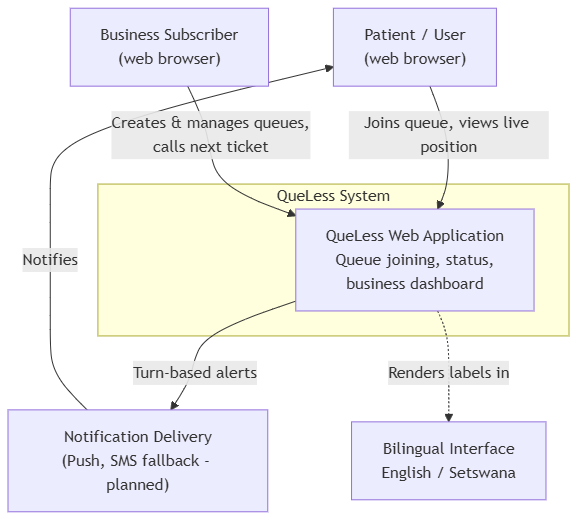
\includegraphics[width=6.00833in,height=5.41667in]{./media/image1.png}

\emph{\textbf{Figure 1: QueLess System Context Diagram}}

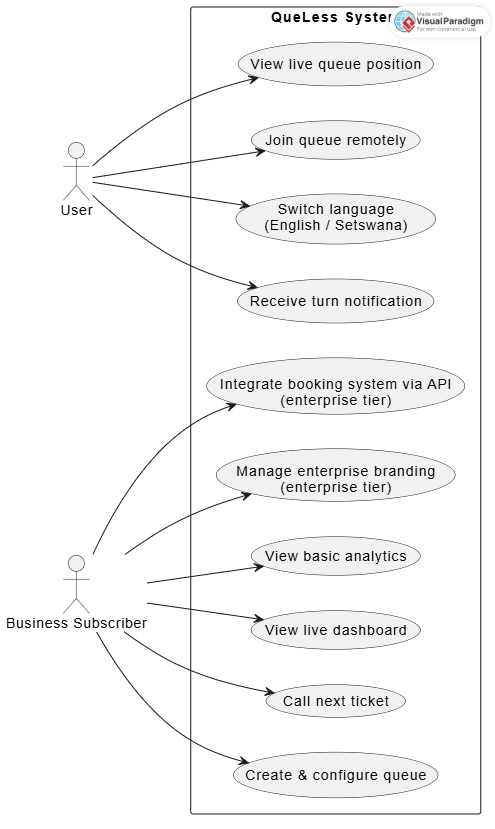
\includegraphics[width=5.15833in,height=8.63333in]{./media/image2.png}

\emph{\textbf{Figure 2: QueLess Core Use Case Diagram}}

\subsection{3.3 Entity Relationship Diagram
(ERD)}\label{entity-relationship-diagram-erd}

The ERD models the core data required by QueLess. A User can hold
multiple tickets, a Business can operate multiple queues, and each Queue
can contain multiple tickets. Each ticket represents a
user\textquotesingle s position in a particular queue and can generate
one or more notifications. Foreign keys provide the relationships
between these entities.

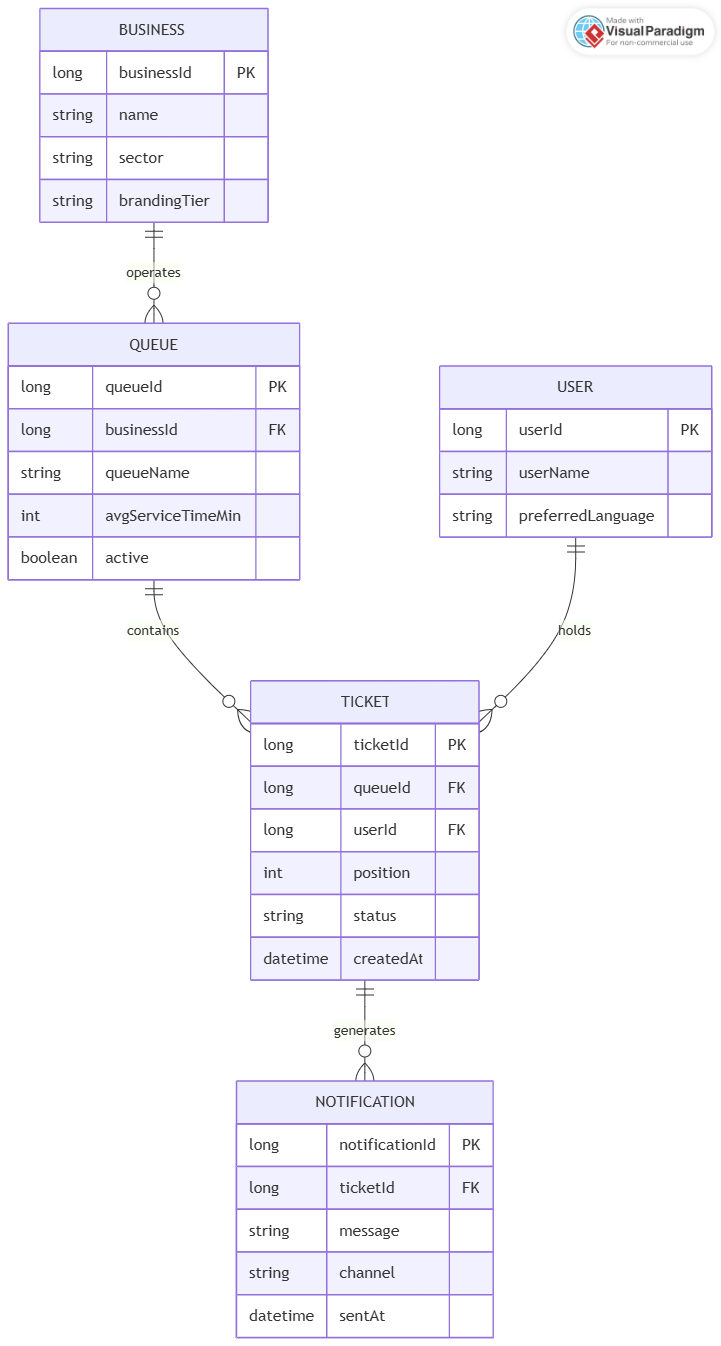
\includegraphics[width=5.08611in,height=9.5in]{./media/image3.png}

\emph{\textbf{Figure 3: QueLess Entity Relationship Diagram}}

\subsection{3.4 Class Diagrams}\label{class-diagrams}

The UML class view separates queue operations, notifications, dashboard
functions and core data objects. QueueManager is responsible for queue
operations, NotificationService handles turn alerts and fallback
notification behaviour, while DashboardActivity (labelled in Figure 4,
produced before the implementation technology was finalised) represents
business-facing queue-management functions. In the Java web
implementation described in Section 4, this responsibility is carried
out by DashboardServlet together with dashboard.jsp; the class diagram
should be relabelled to reflect this the next time the diagrams are
regenerated.

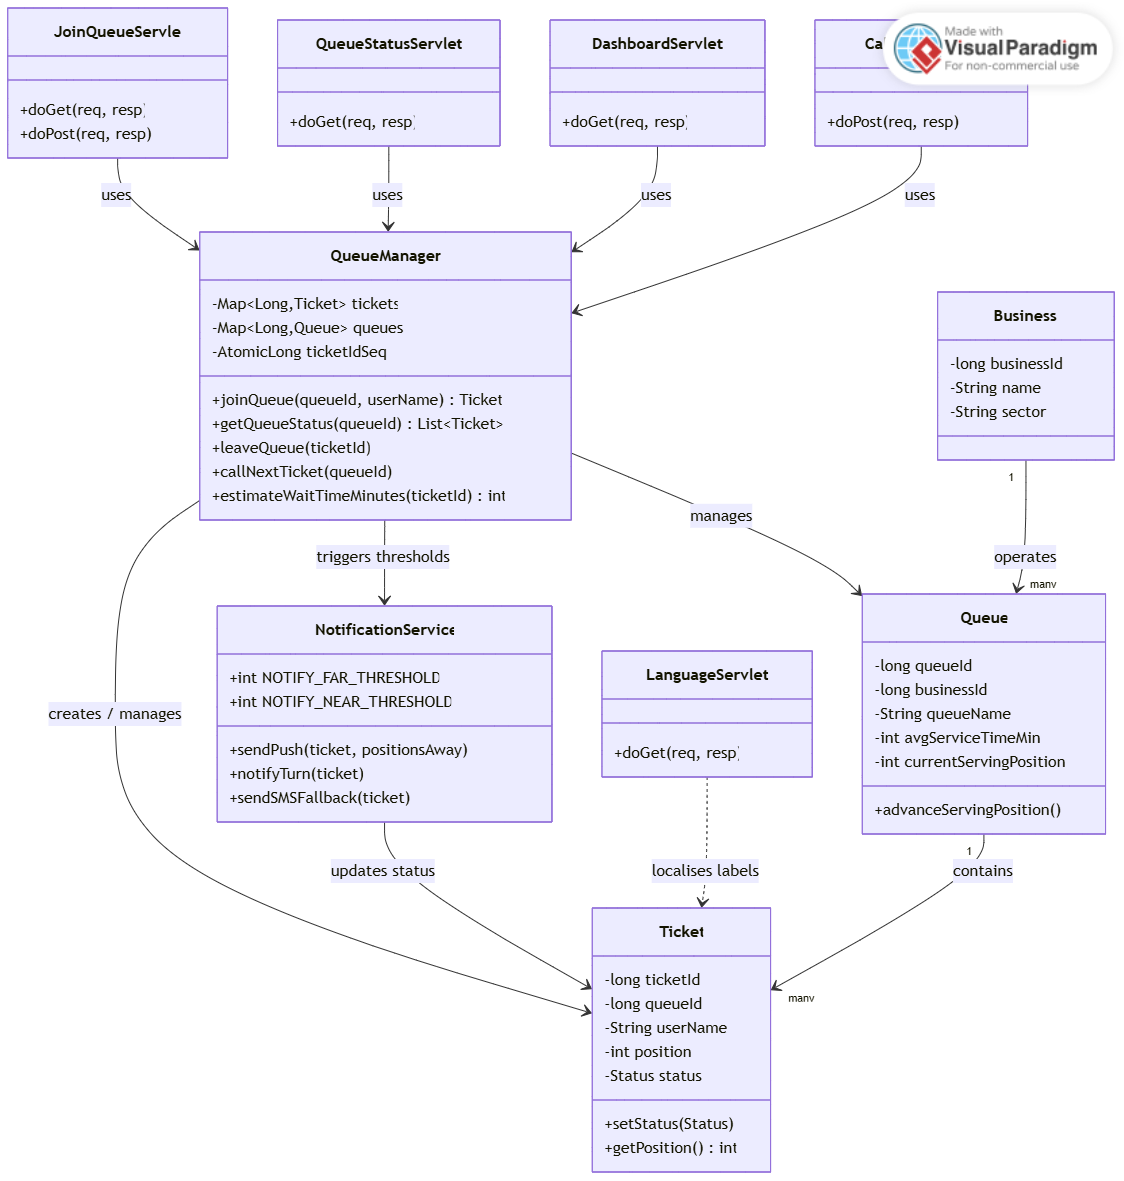
\includegraphics[width=6.8in,height=7.14375in]{./media/image4.png}

\emph{\textbf{Figure 4: QueLess UML Class Diagram}}

The process below shows the principal user journey from joining a queue
to being called for service.

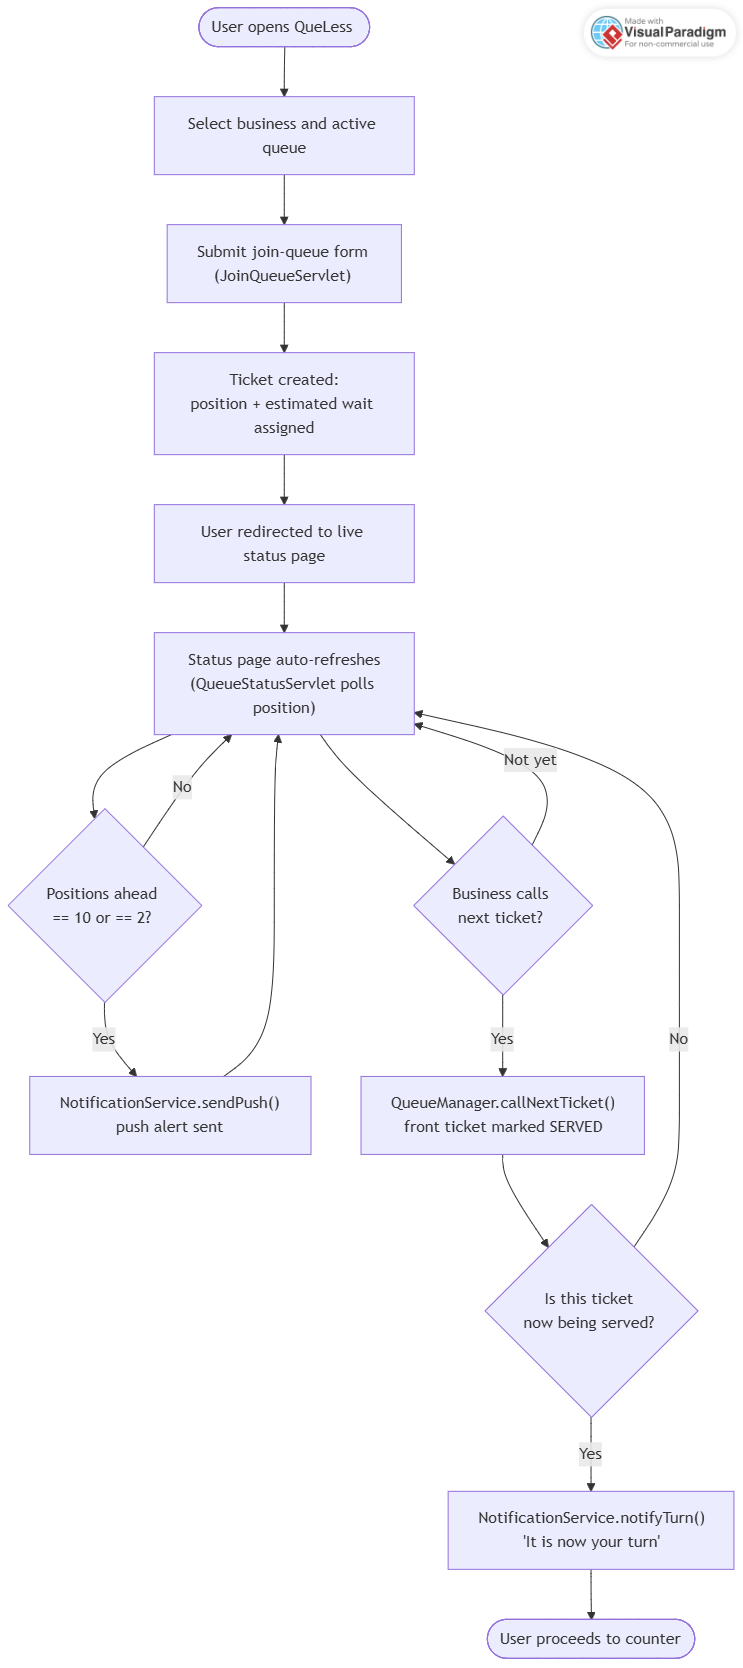
\includegraphics[width=4.23264in,height=9.5in]{./media/image5.png}

\emph{\textbf{Figure 5: QueLess Queue Joining and Notification Flow}}

\subsection{3.5 Dashboard Design}\label{dashboard-design}

The dashboard is designed around live operational information. Summary
cards provide a quick view of active queues, waiting patients, average
waiting time and tickets served. The live queue monitor supports actions
such as calling the next ticket, while the analytics area provides a
simple view of demand trends. The layout is intended to reduce the
number of steps required by business staff during busy periods.

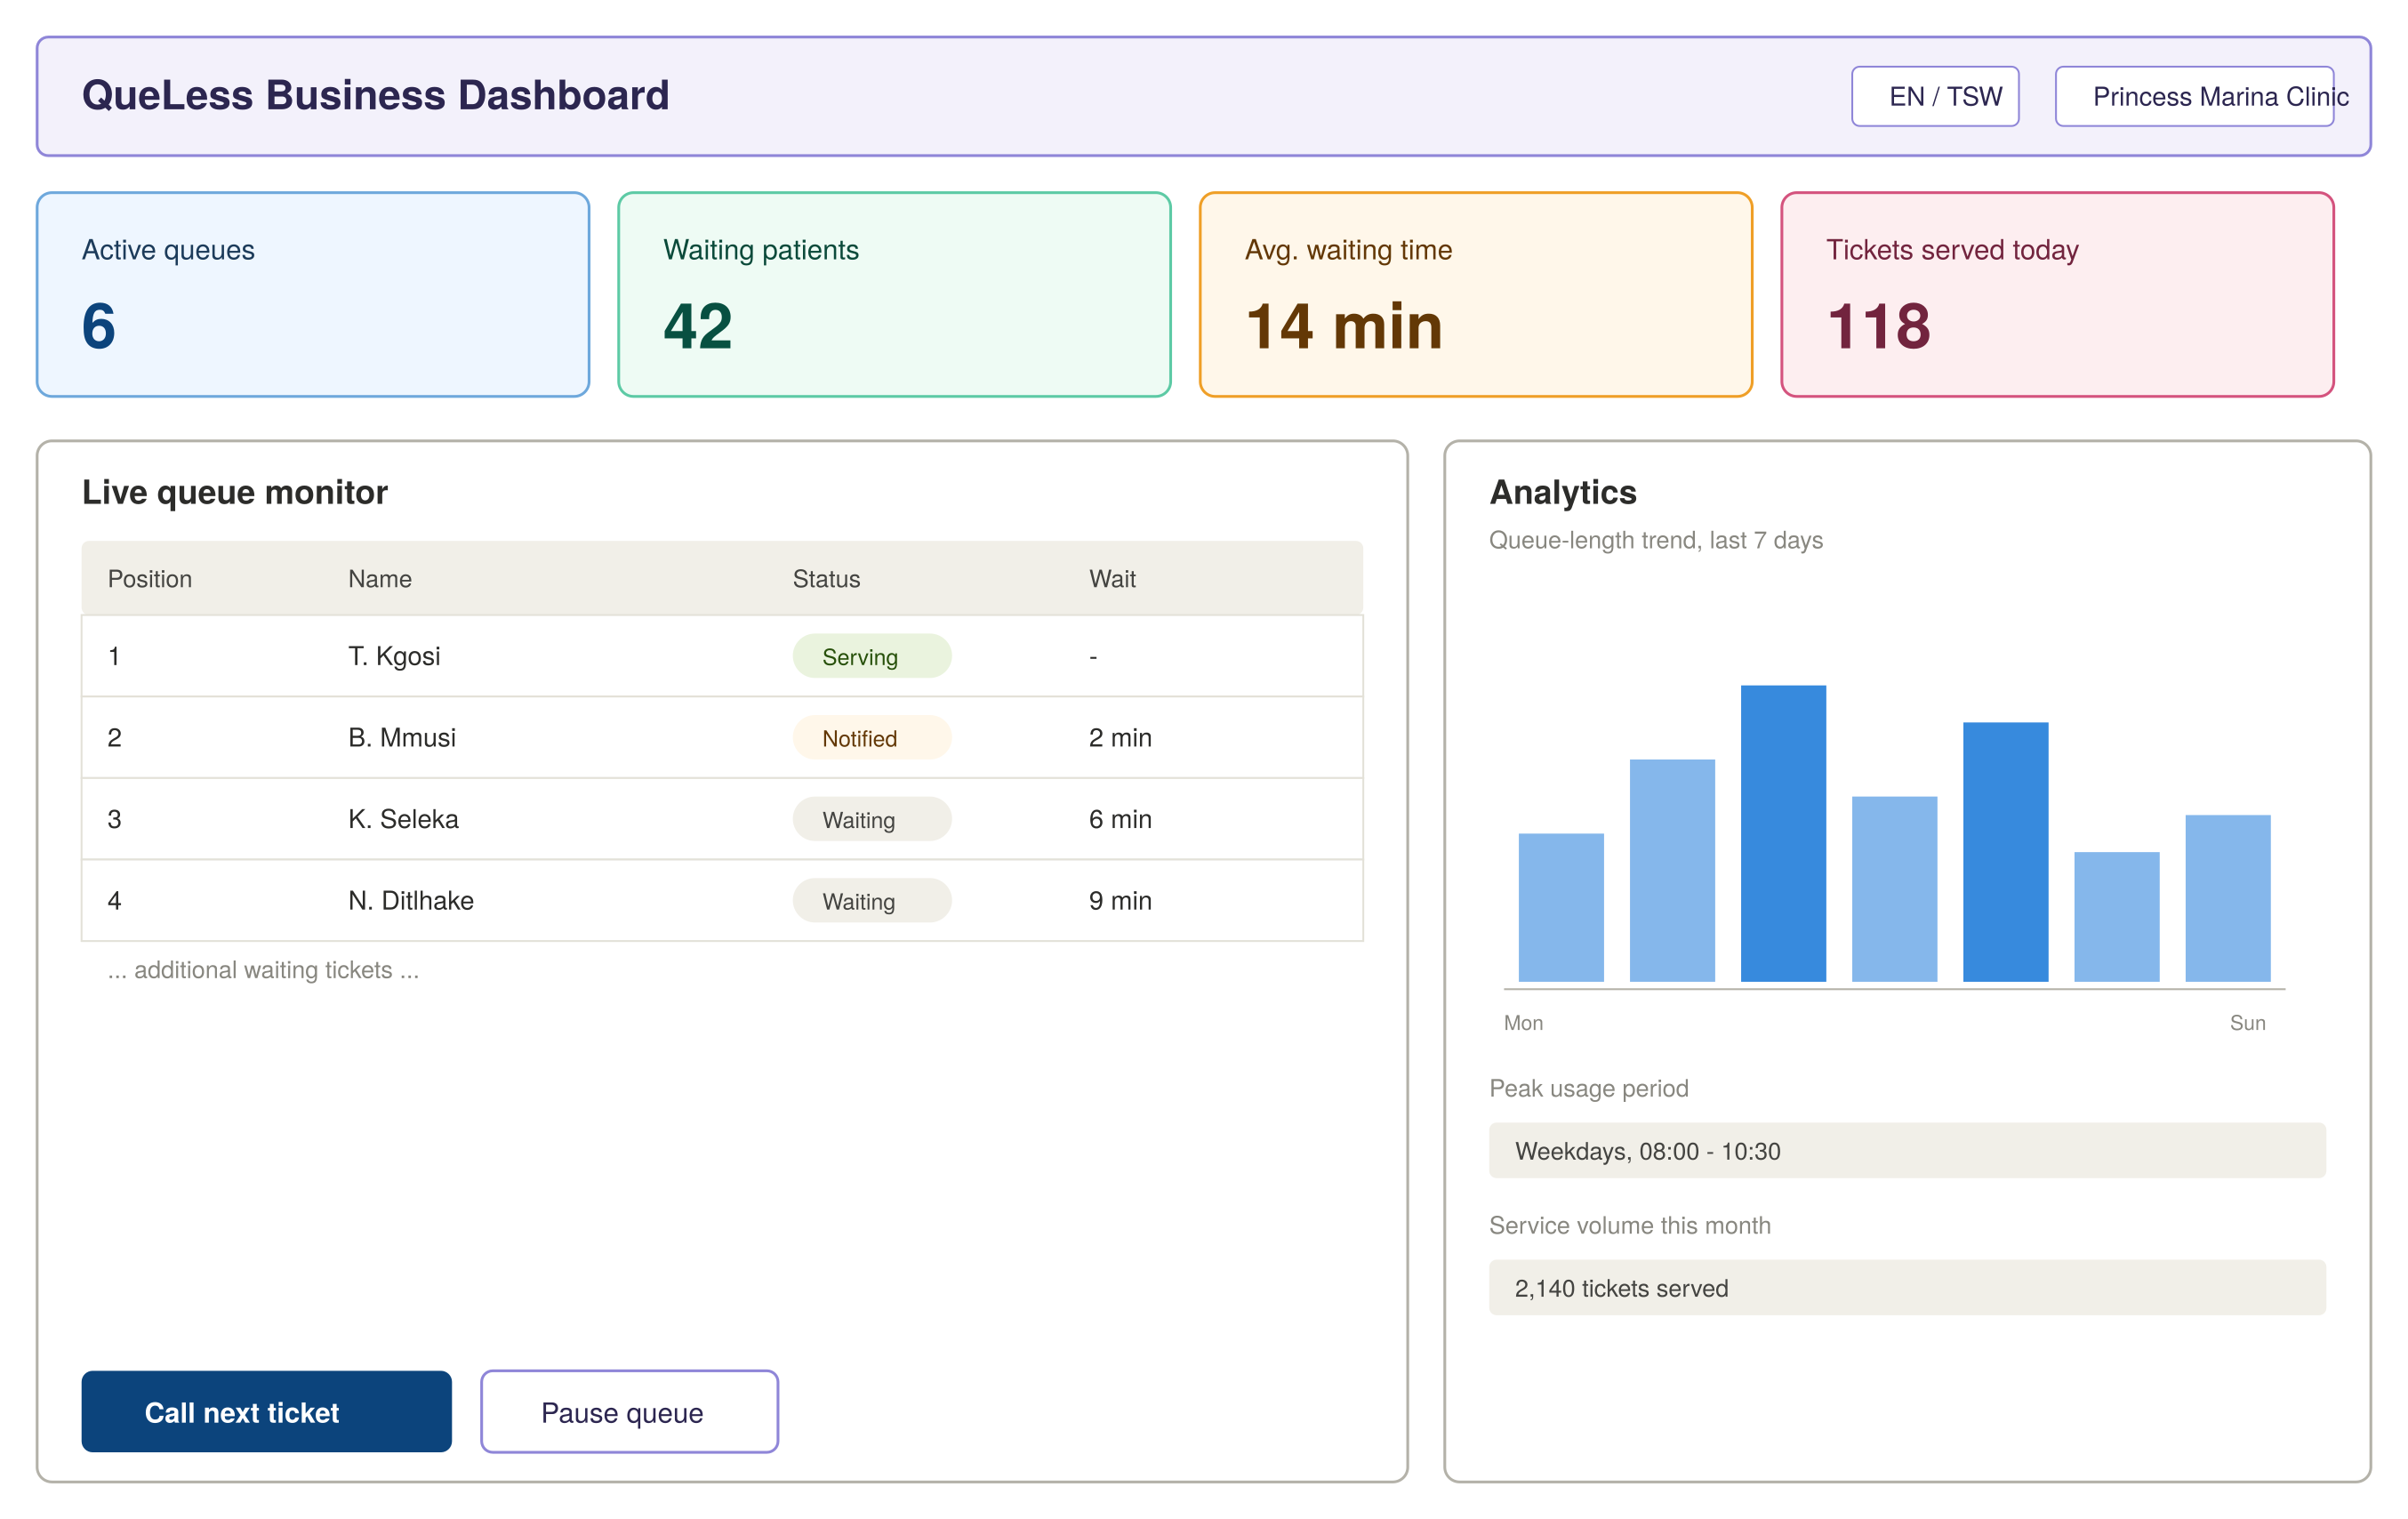
\includegraphics[width=6.8in,height=4.28819in]{./media/image6.png}

\emph{\textbf{Figure 6: Business Dashboard Wireframe}}

\section{4. Implementation}\label{implementation}

The implementation uses Java (Jakarta EE 11) with Servlets and JSP,
built with Maven and developed in IntelliJ IDEA, deployed to Apache
Tomcat 11. This aligns QueLess with the same Jakarta EE toolchain used
elsewhere in the student\textquotesingle s coursework, and lets both the
user-facing queue-joining pages and the business-facing dashboard be
delivered and demonstrated through an ordinary web browser rather than
requiring an installed mobile app. QueueManager provides the central
queue operations as a single, application-wide shared instance
(registered via a ServletContextListener), NotificationService manages
turn-based notifications and the defined SMS fallback, and a set of
Servlets (JoinQueueServlet, QueueStatusServlet, DashboardServlet,
CallNextServlet, LanguageServlet) together with their JSP views replace
the single DashboardActivity concept from the original Android-oriented
design.

The main implementation flow is business and queue selection → ticket
creation via a submitted form → position and estimated waiting-time
calculation → queue monitoring via automatic page refresh → turn
notification → service completion. Queue state is updated whenever a
ticket is created, served or cancelled. The estimated waiting time is
calculated from the number of positions ahead multiplied by the average
service time maintained for the selected queue. User authentication
(login) is not yet implemented in this MVP - any name can currently be
entered when joining a queue - and is listed as a near-term gap in
Section 5.1.

Data protection is treated as a design requirement rather than an
optional feature. User information should be limited to what is
necessary for queue operation, access should be controlled through
authentication and data should be protected in transit and at rest. The
bilingual interface should provide English and Setswana labels without
changing the underlying queue logic.

Implementation challenges include maintaining consistent queue positions
when several users join at nearly the same time, delivering
notifications reliably without a persistent connection to the browser,
supporting a range of browsers and lower-powered devices, and preventing
unauthorised access to business queue information. The current MVP
addresses concurrent joins using thread-safe in-memory collections
(ConcurrentHashMap) inside QueueManager, and approximates real-time
notification delivery with a short automatic page refresh on the status
and dashboard pages rather than a persistent push connection. These
remain areas for further work: notification retry/fallback behaviour, a
real (non-refresh-based) push mechanism such as WebSocket or Server-Sent
Events, and role-based access control are not yet implemented.

\subsection{4.1 Implementation Module
Responsibilities}\label{implementation-module-responsibilities}

{\def\LTcaptype{none} % do not increment counter
\begin{longtable}[]{@{}
  >{\raggedright\arraybackslash}p{(\linewidth - 4\tabcolsep) * \real{0.3333}}
  >{\raggedright\arraybackslash}p{(\linewidth - 4\tabcolsep) * \real{0.3333}}
  >{\raggedright\arraybackslash}p{(\linewidth - 4\tabcolsep) * \real{0.3333}}@{}}
\toprule\noalign{}
\begin{minipage}[b]{\linewidth}\raggedright
Module/Class
\end{minipage} & \begin{minipage}[b]{\linewidth}\raggedright
Main responsibility
\end{minipage} & \begin{minipage}[b]{\linewidth}\raggedright
Key functions
\end{minipage} \\
\midrule\noalign{}
\endhead
\bottomrule\noalign{}
\endlastfoot
QueueManager & Queue operations and state management (shared
application-wide instance) & joinQueue(), getQueueStatus(),
leaveQueue(), callNextTicket(), estimateWaitTimeMinutes() \\
NotificationService & Turn-based notifications & sendPush(),
notifyTurn(), sendSMSFallback() {[}stub, RQ06 not yet implemented{]} \\
JoinQueueServlet & Lists available queues and handles join requests
(RQ01) & doGet(), doPost() \\
QueueStatusServlet & Serves the user\textquotesingle s live position and
notification state (RQ02) & doGet() \\
DashboardServlet & Business-facing queue view (RQ03) & doGet() \\
CallNextServlet & Advances the queue when the business calls the next
ticket (RQ03) & doPost() \\
LanguageServlet & Switches the interface between English and Setswana
(RQ05) & doGet() \\
Business / Queue / Ticket & Core data objects (Java classes) & Business
details, queue configuration, ticket position and status \\
In-memory data store & Shared application-wide persistence inside
QueueManager (ConcurrentHashMap) & Store and retrieve queue data for all
servlets; to be replaced with a real database in a later phase \\
\end{longtable}
}

The Code Listing section at the front of this report now contains
annotated excerpts taken directly from the implemented Java classes
(QueueManager, NotificationService, JoinQueueServlet), rather than
placeholders. As implementation continues, further excerpts (e.g.
DashboardServlet, the JSP views) can be added in the same style.

\section{5. Testing and Discussions}\label{testing-and-discussions}

Testing is structured around functional correctness, performance,
usability and adoption. The following test matrix converts the project
requirements into observable checks. The performance targets are taken
directly from the requirement catalogue. Actual pass/fail results should
be recorded after the implemented application is executed.

{\def\LTcaptype{none} % do not increment counter
\begin{longtable}[]{@{}
  >{\raggedright\arraybackslash}p{(\linewidth - 8\tabcolsep) * \real{0.1934}}
  >{\raggedright\arraybackslash}p{(\linewidth - 8\tabcolsep) * \real{0.1947}}
  >{\raggedright\arraybackslash}p{(\linewidth - 8\tabcolsep) * \real{0.1944}}
  >{\raggedright\arraybackslash}p{(\linewidth - 8\tabcolsep) * \real{0.2234}}
  >{\raggedright\arraybackslash}p{(\linewidth - 8\tabcolsep) * \real{0.1939}}@{}}
\toprule\noalign{}
\begin{minipage}[b]{\linewidth}\raggedright
ID
\end{minipage} & \begin{minipage}[b]{\linewidth}\raggedright
Test scenario
\end{minipage} & \begin{minipage}[b]{\linewidth}\raggedright
Expected result
\end{minipage} & \begin{minipage}[b]{\linewidth}\raggedright
Measure
\end{minipage} & \begin{minipage}[b]{\linewidth}\raggedright
Status
\end{minipage} \\
\midrule\noalign{}
\endhead
\bottomrule\noalign{}
\endlastfoot
TC01 & Authenticate and open the application & Valid user reaches
queue-selection screen & Authentication success & To execute \\
TC02 & Select an active queue and join remotely & Ticket is created with
position and estimated wait & Position accuracy & To execute \\
TC03 & Change queue position & User view reflects the change within 5
seconds & Latency ≤ 5 s & To execute \\
TC04 & Approach turn threshold & Push notification is generated &
Delivery normally ≤ 10 s & To execute \\
TC05 & Push delivery unavailable & Fallback notification process is
triggered where supported & Graceful degradation & To execute \\
TC06 & Business creates and manages a queue & Queue appears and can be
managed & Functional correctness & To execute \\
TC07 & Business calls next ticket & Next eligible ticket is selected and
queue advances & Correct ordering & To execute \\
TC08 & Switch interface to Setswana & Supported labels change to
Setswana & Language completeness & To execute \\
TC09 & Attempt unauthorised access & Protected information is not
exposed & Access control & To execute \\
TC10 & Run in a browser on a lower-powered device & Core pages remain
usable & Compatibility/usability & To execute \\
\end{longtable}
}

\subsection{5.1 Discussion}\label{discussion}

Successful remote queue joining is expected to reduce the need for
patients to remain physically in waiting areas, while real-time
notifications should reduce uncertainty about when service will occur.
For business subscribers, live queue information and basic analytics
should improve visibility of demand and support better allocation of
staff during peak periods. These expected benefits are consistent with
the literature reviewed in Section 2.

The main limitation at this stage is evidential: executed test logs,
measured notification timings, screenshots and a completed production
deployment have not yet been recorded. Therefore, the test matrix is an
evaluation framework rather than claimed empirical results. Further
evaluation should include multiple browsers and devices, weak-network
conditions, concurrent queue joins and usability feedback from
representative patients and service staff.

The TAM framework provides a useful interpretation of likely user
acceptance. The primary survey reported that 90 percent of respondents
considered the proposed application very useful and 84 percent indicated
that they would use a digital queue-management application. These
findings suggest strong perceived usefulness, but continued adoption
will also depend on ease of use, reliability, notification accuracy and
trust in data handling.

\section{6. Conclusion}\label{conclusion}

QueLess was proposed as a locally relevant smart queue-management system
for healthcare services in Botswana. The project addresses the problem
of long and uncertain waiting times by allowing users to join queues
remotely, monitor their positions and receive turn-based notifications.
A business dashboard provides service providers with a mechanism for
creating, monitoring and managing queues.

The completed analysis and design defines the main actors, use cases,
data entities, software classes, queue flow and dashboard structure. The
design also incorporates the project\textquotesingle s stated
requirements for English and Setswana support, secure handling of user
information and future SMS, analytics, enterprise branding and API
capabilities. The literature review and primary survey provide support
for the relevance and potential acceptance of the concept.

Future development should prioritise completion and validation of the
working web prototype - including user authentication and a real
database in place of the current in-memory store - followed by SMS
fallback, a native mobile application for Android and iOS, stronger
analytics and enterprise integration. Pilot testing with healthcare
facilities would provide evidence about real waiting-time reduction,
staff workload, patient satisfaction and adoption. Expansion to banks,
government offices, retail outlets and other service environments can
then be considered after the healthcare use case has been validated.

\section{References}\label{references}

Alrasheedi, K.F., Al-Mohaithef, M., Edrees, H.H. and Chandramohan, S.
(2019) \textquotesingle The association between wait times and patient
satisfaction: findings from primary health centers in the Kingdom of
Saudi Arabia\textquotesingle, Health Services Research and Managerial
Epidemiology, 6.

BOCRA (2023) Annual Report 2022/2023. Gaborone: Botswana Communications
Regulatory Authority.

BOCRA (2025) Annual Report 2024/2025. Gaborone: Botswana Communications
Regulatory Authority.

BW Tech Zone (2026) \textquotesingle Starlink has over 8,000 customers
in Botswana\textquotesingle. Available at:
https://www.bwtechzone.com/2026/07/starlink-has-over-8000-customers-in.html
(Accessed: 27 August 2026).

Daily News (2026a) \textquotesingle Inside Botswana\textquotesingle s
health crisis\textquotesingle. Gaborone: Botswana Government Daily News.
Available at: https://dailynews.gov.bw/news-detail/89709 (Accessed: 27
August 2026).

Daily News (2026b) \textquotesingle Govt acts to decongest Princess
Marina\textquotesingle. Gaborone: Botswana Government Daily News.
Available at: https://dailynews.gov.bw/news-detail/89761 (Accessed: 27
August 2026).

DataReportal (2026) Digital 2026: Botswana. Available at:
https://datareportal.com/reports/digital-2026-botswana (Accessed: 27
August 2026).

Davis, F.D., Bagozzi, R.P. and Warshaw, P.R. (1989)
\textquotesingle User acceptance of computer technology: a comparison of
two theoretical models\textquotesingle, Management Science, 35(8), pp.
982--1003.

Ekow Kelly, A. and Palaniappan, S. (2023) \textquotesingle Using a
technology acceptance model to determine factors influencing continued
usage of mobile money service transactions in Ghana\textquotesingle,
Journal of Innovation and Entrepreneurship, 12(34).

Garedew, B.T., Azene, D.K., Jilcha, K. and Betizazu, S.S. (2024)
\textquotesingle Machine learning based lean service quality improvement
by reducing waiting time in the healthcare sector\textquotesingle,
International Journal of Quality and Reliability Management.

Gokulakrishnan, A. (2023) \textquotesingle Role of virtual queue
management system in improving service efficiency in banks at Chennai
city\textquotesingle, Academic Leadership (Online Journal).

Maister, D.H. (1985) \textquotesingle The psychology of waiting
lines\textquotesingle, in Czepiel, J.A., Solomon, M.R. and Surprenant,
M.R. (eds.) The Service Encounter: Managing Employee or Customer
Interaction in Service Businesses. Lexington: Lexington Books.

McIntyre, D. and Chow, C.K. (2020) \textquotesingle Waiting time as an
indicator for health services under strain: a narrative
review\textquotesingle, Medical Care Research and Review.

Office of the Ombudsman (2026) Under Strain: Inside
Botswana\textquotesingle s Public Health Care Crisis. Gaborone: Office
of the Ombudsman, cited in Daily News (2026a).

PMC (2025) Systematic review of technology use by health workers in low-
and lower-middle-income countries.

QueLess Research Group (2026) Questionnaire Report: Feedback on the
QueLess App {[}Primary research survey of 50 participants{]}. Gaborone:
Botswana School of Business Sciences.

Republic of Botswana (2018) Data Protection Act, 2018. Gaborone:
Government Printer.

The Voice (2025) \textquotesingle Mobile Money madness!\textquotesingle.
Available at: https://thevoicebw.com/mobile-money-madness/ (Accessed: 27
August 2026).

UNDP (2026) Digital and AI can help people live healthier lives.
Available at:
https://www.undp.org/digital-and-ai-can-help-people-live-healthier-lives
(Accessed: 26 August 2026).

Worldometer (2026) Botswana Population. Available at:
https://www.worldometers.info/world-population/botswana-population
(Accessed: 27 August 2026).

\section{Appendices}\label{appendices}

\subsection{Appendix A: Requirement
Catalogue}\label{appendix-a-requirement-catalogue}

\subsubsection{RQ01 -- A user must be able to join a service queue
remotely.}\label{rq01-a-user-must-be-able-to-join-a-service-queue-remotely.}

Requirement: A user must be able to join a service queue remotely.

Requirement ID: RQ01

Requirement Description: The system shall allow an authenticated user to
select a business and active queue, reserve a position without being
physically present and receive confirmation of the queue position and
estimated waiting time.

Non-functional requirements: Queue position should update within 5
seconds; the interface should remain usable in common web browsers and
on lower-powered devices; data should be protected in transit and at
rest.

\subsubsection{RQ02 -- A user must be notified as their turn
approaches.}\label{rq02-a-user-must-be-notified-as-their-turn-approaches.}

Requirement: A user must be notified as their turn approaches.

Requirement ID: RQ02

Requirement Description: The system shall notify the user at
configurable thresholds, such as 10 and 2 positions before service, and
again when it is their turn.

Non-functional requirements: Notifications should normally be delivered
within 10 seconds; failed push delivery should degrade gracefully to SMS
where available.

\subsubsection{RQ03 -- A business must be able to create, manage and
monitor
queues.}\label{rq03-a-business-must-be-able-to-create-manage-and-monitor-queues.}

Requirement: A business must be able to create, manage and monitor
queues.

Requirement ID: RQ03

Requirement Description: The dashboard shall allow an authorised
business subscriber to create queues, configure service details,
pause/resume queues, view waiting tickets and call the next eligible
ticket.

Non-functional requirements: Dashboard actions should be role-protected
and queue changes should be reflected consistently.

\subsubsection{RQ04 -- User and queue data must be stored
securely.}\label{rq04-user-and-queue-data-must-be-stored-securely.}

Requirement: User and queue data must be stored securely.

Requirement ID: RQ04

Requirement Description: The system shall authenticate users, restrict
access to authorised information and protect stored and transmitted data
in line with the Botswana Data Protection Act (2018).

Non-functional requirements: Data minimisation, controlled access and
encryption should be applied; unauthorised users must not access
protected queue information.

\subsubsection{RQ05 -- The interface must support English and
Setswana.}\label{rq05-the-interface-must-support-english-and-setswana.}

Requirement: The interface must support English and Setswana.

Requirement ID: RQ05

Requirement Description: The system shall provide equivalent core
navigation and queue-management labels in English and Setswana.

Non-functional requirements: Language switching should not change
underlying queue data or business logic.

\subsubsection{RQ06 -- The system should provide SMS notification
fallback.}\label{rq06-the-system-should-provide-sms-notification-fallback.}

Requirement: The system should provide SMS notification fallback.

Requirement ID: RQ06

Requirement Description: Where smartphone data or push delivery is
unreliable, the system should support an SMS-based notification option
for eligible users.

Non-functional requirements: Fallback should be triggered gracefully and
should not create duplicate or contradictory turn information.

\subsubsection{RQ07 -- The system should provide basic business
analytics.}\label{rq07-the-system-should-provide-basic-business-analytics.}

Requirement: The system should provide basic business analytics.

Requirement ID: RQ07

Requirement Description: The dashboard should present queue-length
trends, peak usage periods, waiting-time indicators and service-volume
summaries.

Non-functional requirements: Reports should be understandable, generated
from stored queue events and limited to authorised business data.

\subsubsection{RQ08 -- Enterprise subscribers should support custom
branding.}\label{rq08-enterprise-subscribers-should-support-custom-branding.}

Requirement: Enterprise subscribers should support custom branding.

Requirement ID: RQ08

Requirement Description: Enterprise accounts should be able to configure
approved organisation branding such as name, logo and interface
identity.

Non-functional requirements: Branding changes should be isolated to the
relevant organisation and should not alter core system functions.

\subsubsection{RQ09 -- Enterprise clients should support API
integration.}\label{rq09-enterprise-clients-should-support-api-integration.}

Requirement: Enterprise clients sh-ould support API integration.

Requirement ID: RQ09

Requirement Description: The system should provide an integration layer
through which approved enterprise clients can connect existing booking
systems to QueLess queue operations.

Non functional requirements: API access should be authenticated,
authorised, documented and protected against invalid or excessive
requests.

\subsection{Appendix B: Additional
Material}\label{appendix-b-additional-material}

The six diagrams in Section 3 form the main supporting design artefacts
for the project (Figure 4 should be relabelled DashboardServlet in place
of DashboardActivity the next time it is regenerated, per the note in
Section 3.4). The final project submission should also include
screenshots of the implemented web application, dashboard screens,
executed test logs, extended survey results and further annotated
source-code excerpts as testing progresses.

\end{document}
